\begin{table}[H]
\centering
\begin{tabular}{| l | l | l |}
\hline
Type & RMSD & Percent \\ \hline
Under & 138 & 89.2\% \\ \hline
Over & 32 & 10.8\% \\ \hline
Total & 131 & \\ \hline
\end{tabular}
\caption{Regression predictor results for the baseline workload}
\end{table}

\begin{figure}[H]
\centering
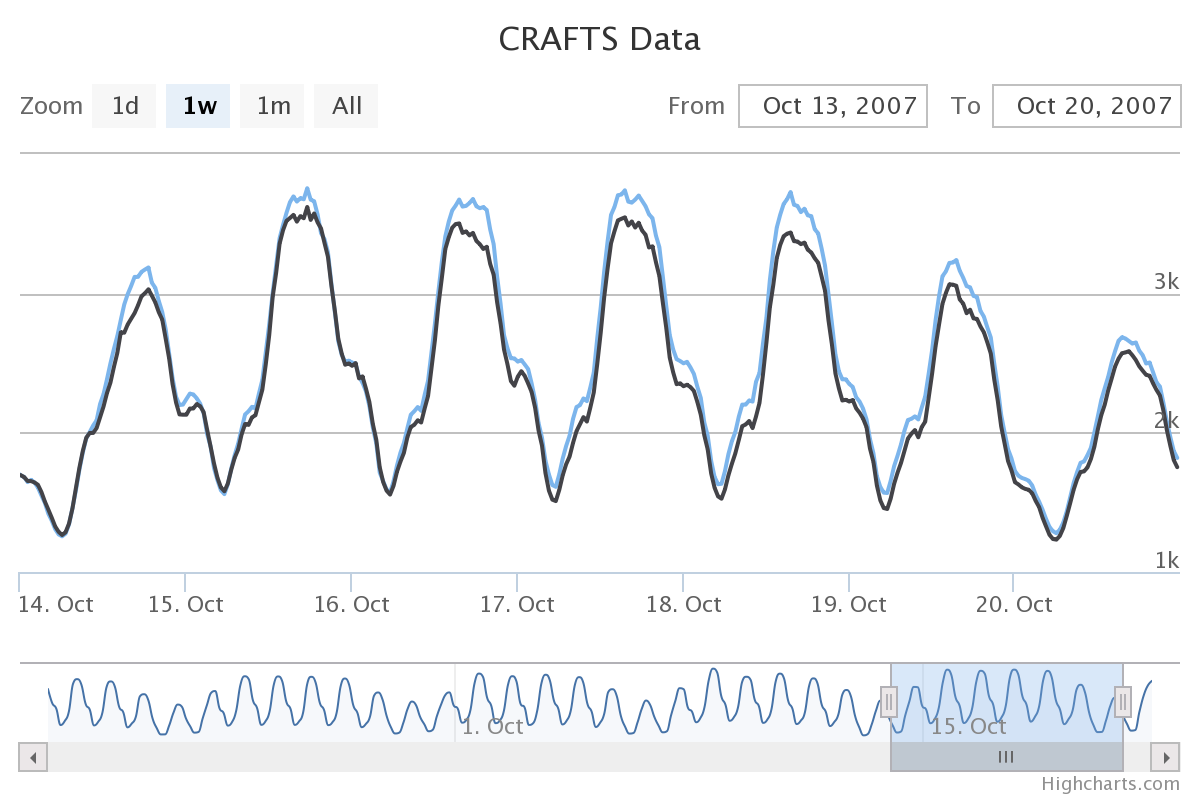
\includegraphics[width=\textwidth]{results/graphs/regression_baseline.png}
\caption{Regression prediction results for the baseline workload}
\label{fig:regression_b}
\end{figure}

\begin{table}[H]
\centering
\begin{tabular}{| l | l | l | l | l |}
\hline
Type & \multicolumn{2}{c |}{Regular} & \multicolumn{2}{c |}{Anomalous} \\ \hline
 & RMSD & Percent & RMSD & Percent \\ \hline
Under & 138 & 89.1\% & 270 & 100.0\% \\ \hline
Over & 32 & 10.9\% & 0 & 0.0\% \\ \hline
Total & 131 & & 270 & \\ \hline
\end{tabular}
\caption{Regression predictor results for the training outage workload}
\end{table}

\begin{figure}[H]
\centering
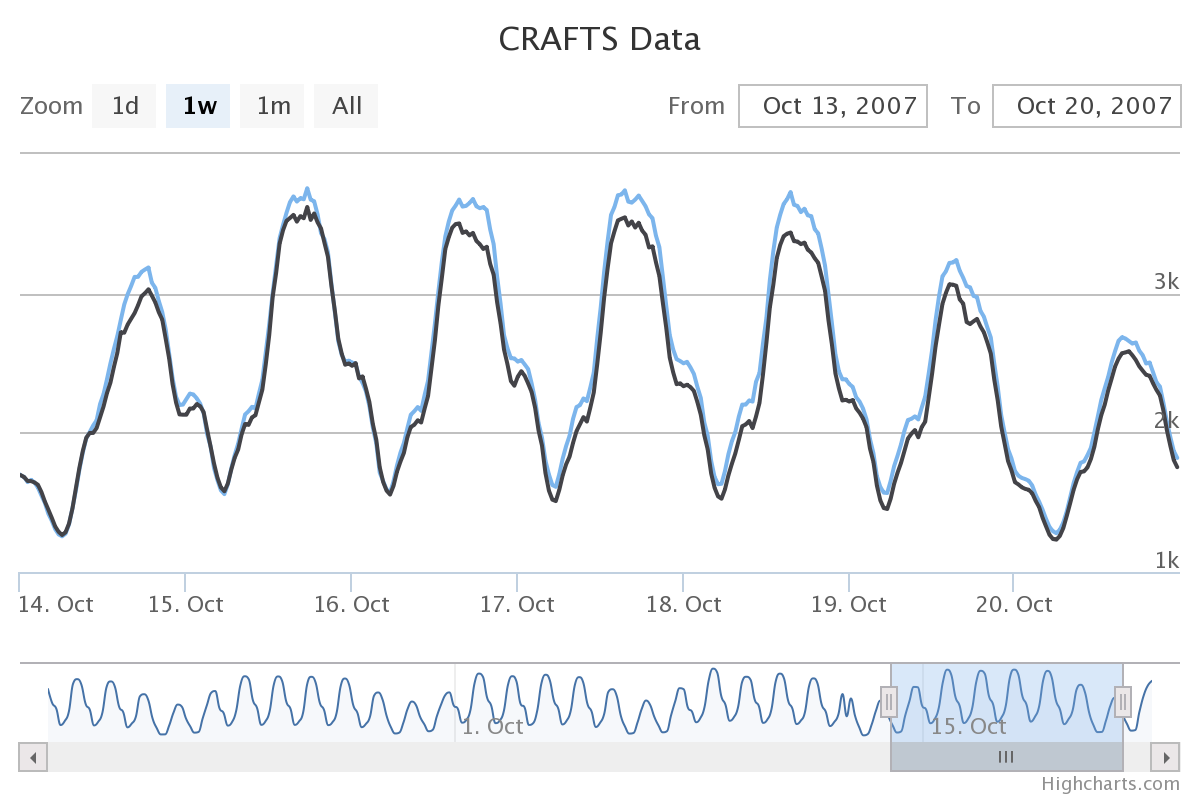
\includegraphics[width=\textwidth]{results/graphs/regression_training_outage.png}
\caption{Regression prediction results for the training outage workload}
\label{fig:regression_to}
\end{figure}

\begin{table}[H]
\centering
\begin{tabular}{| l | l | l | l | l |}
\hline
Type & \multicolumn{2}{c |}{Regular} & \multicolumn{2}{c |}{Anomalous} \\ \hline
 & RMSD & Percent & RMSD & Percent \\ \hline
Under & 138 & 89.0\% & 0 & 0.0\% \\ \hline
Over & 274 & 11.0\% & 2869 & 100.0\% \\ \hline
Total & 159 & & 2869 & \\ \hline
\end{tabular}
\caption{Regression predictor results for the horizon outage workload}
\end{table}

\begin{figure}[H]
\centering
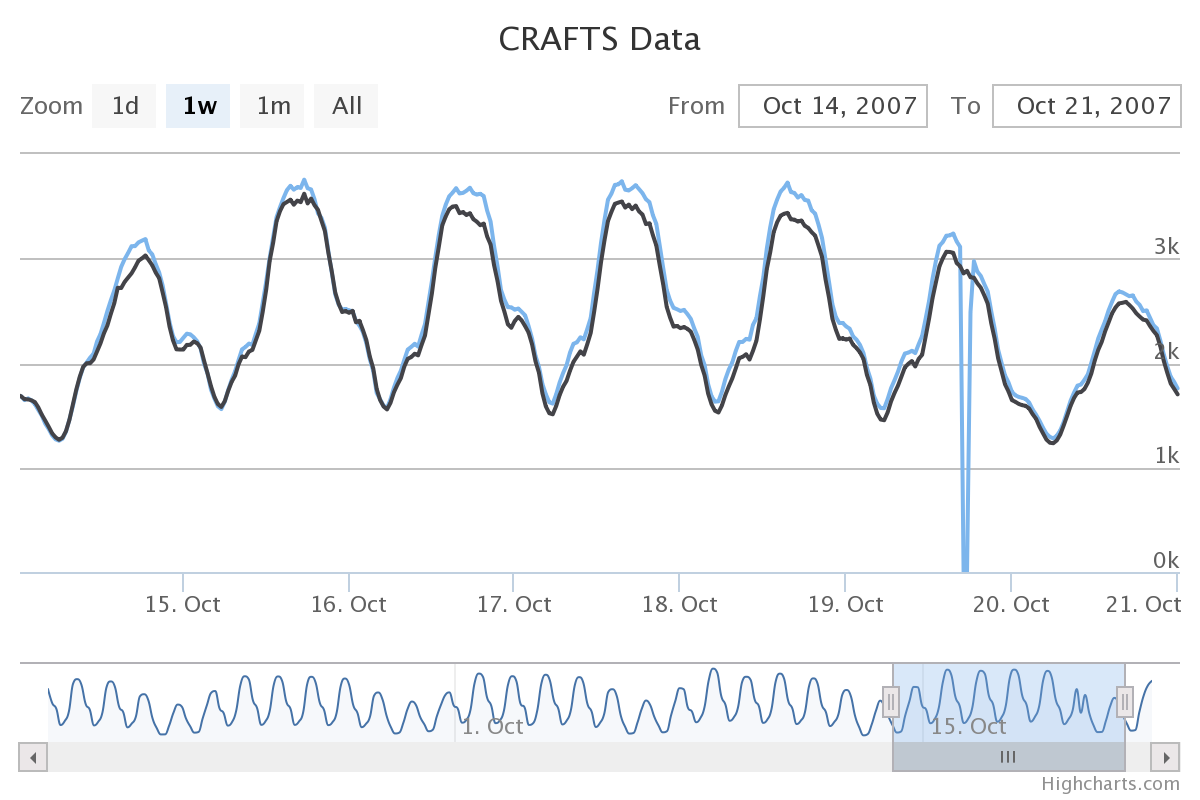
\includegraphics[width=\textwidth]{results/graphs/regression_horizon_outage.png}
\caption{Regression prediction results for the horizon outage workload}
\label{fig:regression_ho}
\end{figure}

\begin{table}[H]
\centering
\begin{tabular}{| l | l | l | l | l |}
\hline
Type & \multicolumn{2}{c |}{Regular} & \multicolumn{2}{c |}{Anomalous} \\ \hline
 & RMSD & Percent & RMSD & Percent \\ \hline
Under & 138 & 89.2\% & 177 & 100.0\% \\ \hline
Over & 32 & 10.8\% & 0 & 0.0\% \\ \hline
Total & 131 & & 177 & \\ \hline
\end{tabular}
\caption{Regression predictor results for the training spike workload}
\end{table}

\begin{figure}[H]
\centering
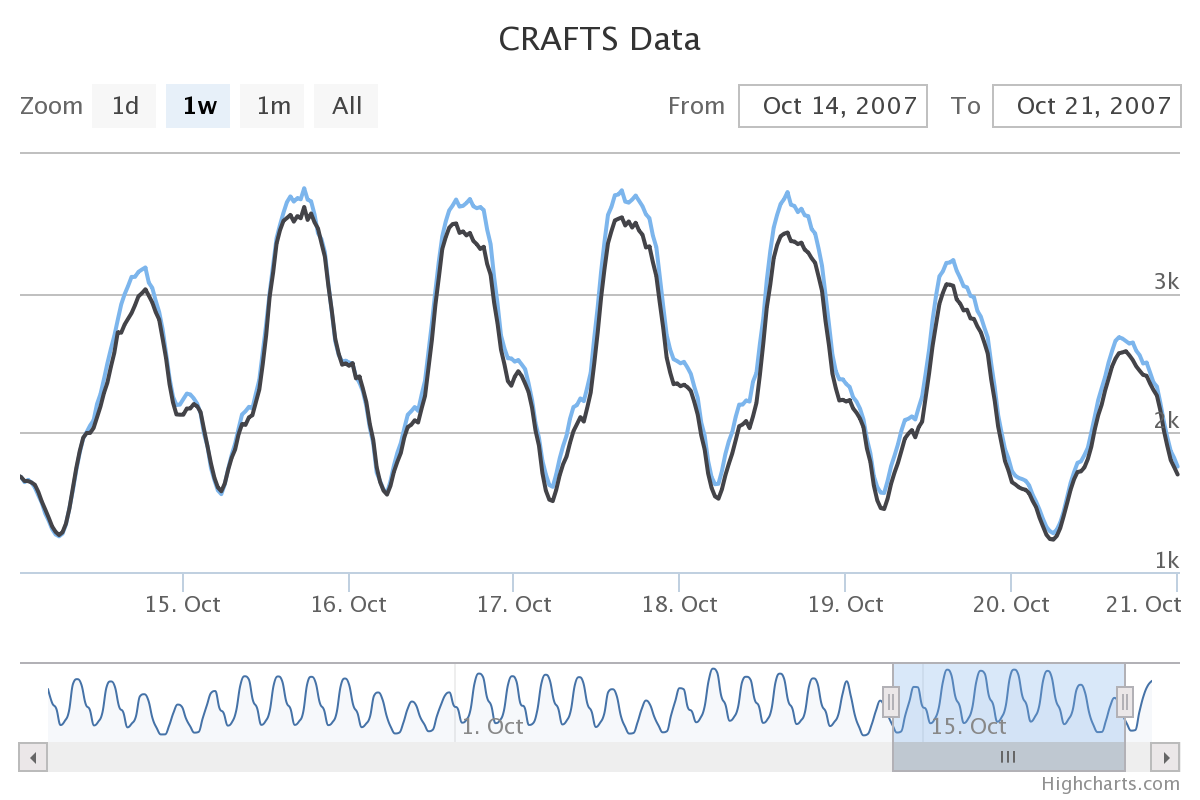
\includegraphics[width=\textwidth]{results/graphs/regression_training_spike.png}
\caption{Regression prediction results for the training spike workload}
\label{fig:regression_ts}
\end{figure}

\begin{table}[H]
\centering
\begin{tabular}{| l | l | l | l | l |}
\hline
Type & \multicolumn{2}{c |}{Regular} & \multicolumn{2}{c |}{Anomalous} \\ \hline
 & RMSD & Percent & RMSD & Percent \\ \hline
Under & 175 & 89.2\% & 3260 & 100.0\% \\ \hline
Over & 32 & 10.8\% & 0 & 0.0\% \\ \hline
Total & 166 & & 3260 & \\ \hline
\end{tabular}
\caption{Regression predictor results for the horizon spike workload}
\end{table}

\begin{figure}[H]
\centering
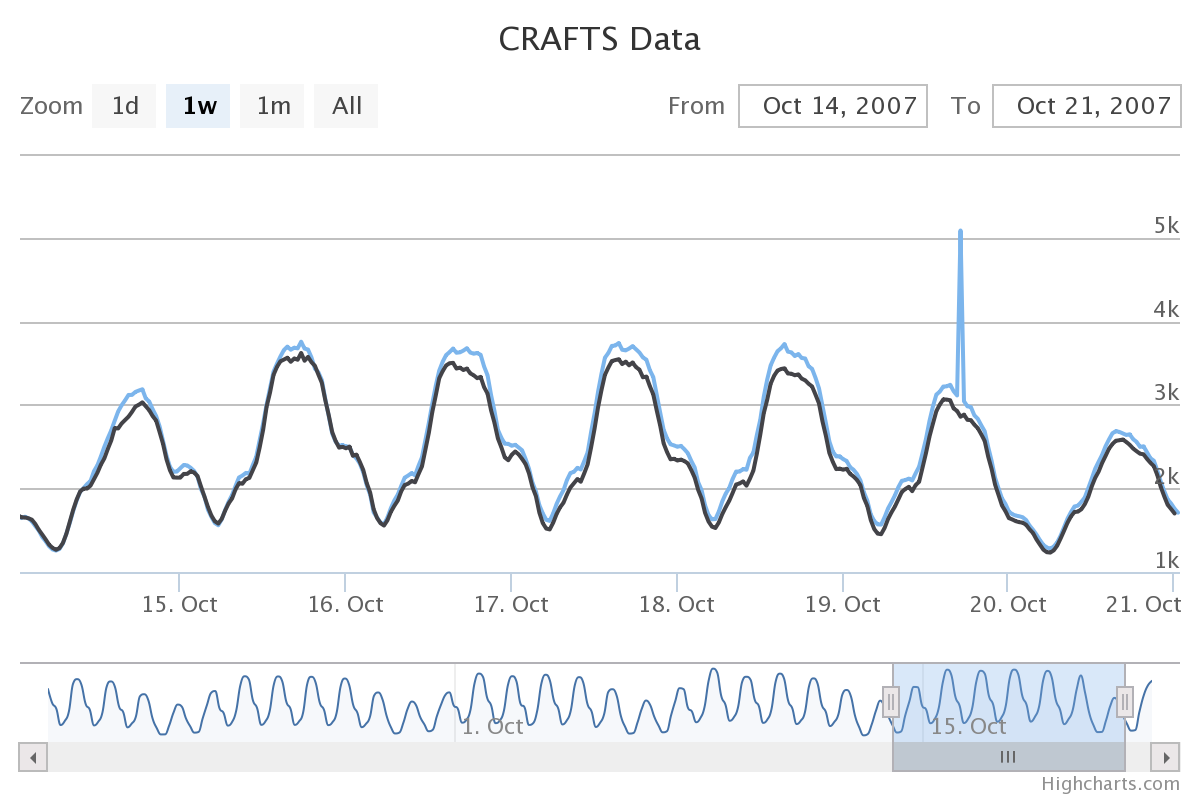
\includegraphics[width=\textwidth]{results/graphs/regression_horizon_spike.png}
\caption{Regression prediction results for the horizon spike workload}
\label{fig:regression_hs}
\end{figure}